\documentclass{article}

\usepackage{ctex}
\usepackage{graphicx}
\usepackage{subfigure}
\usepackage{listings}

\title{二叉搜索树}
\author{Xingdong Xue}
\date{Mar. 2020}

\begin{document}
\maketitle

\section{概念}
\subsection{循关键码访问}

二叉搜索树是一系列根据关键码进行查找的数据项,call-by-key。
其中\textbf{关键码}之间可以比较大小,可以进行相等比对,统一表示和实现为entry的形式。

\subsection{二叉搜索树}

满足顺序性(任一节点不小于其左后代,不大于其右后代)的二叉树。

BST的中序遍历序列,必然单调非降。(充要条件)

\subsection{接口}

除了继承BinTree外,还有以下接口:
\begin{itemize}
  \item search(T):查找
  \item insert(T):插入
  \item delete(T):删除
\end{itemize}

\section{算法与实现}
\subsection{查找}

实质上就是有序向量的二分查找,代码如下:
\begin{lstlisting}[language=Python]
def search(self, e):
  return self.searchIn(self.root, e, hot=None)

def searchIn(self, v, e, hot):
  if not v or e == v.data:
      return v
  hot = v # 记下当前非空节点
  return self.searchIn(v.lChild if e < v.data else v.rChild, e, hot)
\end{lstlisting}

查找成功时,返回一个关键码为e的真实节点;查找失败时,返回一个空节点。

如果在失败时,假想这个空节点为一个数值位e的哨兵节点,则可以得出:返回值总是代表命中节点,而hot的值永远是命中节点的父亲。

算法的时间复杂度为$O(h)$,其中h为树的高度。

\subsection{插入}

根据查找得出的结论,查找的返回值永远为命中节点,则插入就是在查找返回值的位置上新增一个节点即可。
\begin{lstlisting}[language=Python]
def insert(self, e):
  x = self.search(e)
  if not x:
      x = BinNode(e, hot)
  # TODO 更新树的规模,更新祖先的高度
  return x
\end{lstlisting}

算法的时间复杂度为$O(h)$,其中h为树的高度。

\subsection{删除}

\begin{lstlisting}[language=Python]
def remove(self, e):
  x = self.search(e)
  if not x:
      return False
  self.removeAt(x, hot)
  # TODO 更新树的规模,更新祖先的高度
  return True
\end{lstlisting}

函数removeAt分几种情况:
\begin{enumerate}
  \item 至多只有一个孩子:删除节点并用子节点替代。
  \item 左右孩子同时存在:找出直接后继(找到右子树并不断为往左侧下行)并与之交换,然后按照第一种情况删除。
\end{enumerate}

算法的时间复杂度为$O(h)$,其中h为树的高度。

\section{平衡与平均高度}
普通二叉搜索树在数据极端的情况下,可能会退化为单链,导致算法的时间复杂度$O(h) = O(n)$。

所以需要有更客观的方法去分析二叉树操作的平均复杂度。

按照随机生成来估算:$n!$,复杂度为$O(\log_{}n)$
随机组成:卡特兰数,复杂度为$O(\sqrt{n})$

\subsection{理想平衡}
由n各节点组成的高度为$\log_2n$的二叉树,达到\textbf{理想平衡}。

理想平衡的概率极低,且维护成本过高,所以适当放松标准,达到\textbf{适度平衡}。

适度平衡的二叉树,称作平衡二叉搜索树(BBST)。

\subsection{等价变换}

我们将中序遍历序列相同,但拓扑结构不同的BST称作等价BST。

通过等价变换和旋转调整,任何一对等价BST之间的变换都可以通过旋转变换得到。

\section{AVL树}
\subsection{平衡因子}

$$balFac(v) = height(lc(v)) - height(rc(v)))$$

在AV树中,平衡因子小于等于1。

\subsection{适度平衡}

高度为h的AVL树,至少包含$S(h) = fib(h+3) - 1$个节点。
$$h \sim \Omega(\Phi^n) \rightarrow n \sim O(log_{}h)$$

\subsection{接口}
除了继承BST外,还有以下接口:
\begin{itemize}
  \item Balanced(x):是否理想平衡
  \item BalFac(x):平衡因子,左右子树高度之差
  \item 重写insert
  \item 重写remove
  \item 复用search等
\end{itemize}

\subsection{失衡与重平衡}

插入操作会使零到多个祖先节点失衡,其余节点则平衡因子维持原状,因为其余节点的高度与孩子高度都不会改变。
删除操作会使得零到一个祖先会失衡,因为假设删除操作让某一个祖先失衡了,则删除的节点一定处于更短的分支上,所以不会影响此祖先的高度,进而不会影响更上级的节点。

\section{插入}

多个节点失衡,最低者g不会低于x祖父辈。

g经过单旋后复衡,字数高度复原;更高祖先也必平衡,全树复衡。

\subsection{zigzig/zagzag型}
\begin{figure}[htb]
  \centering
  \subfigure[before.]{
    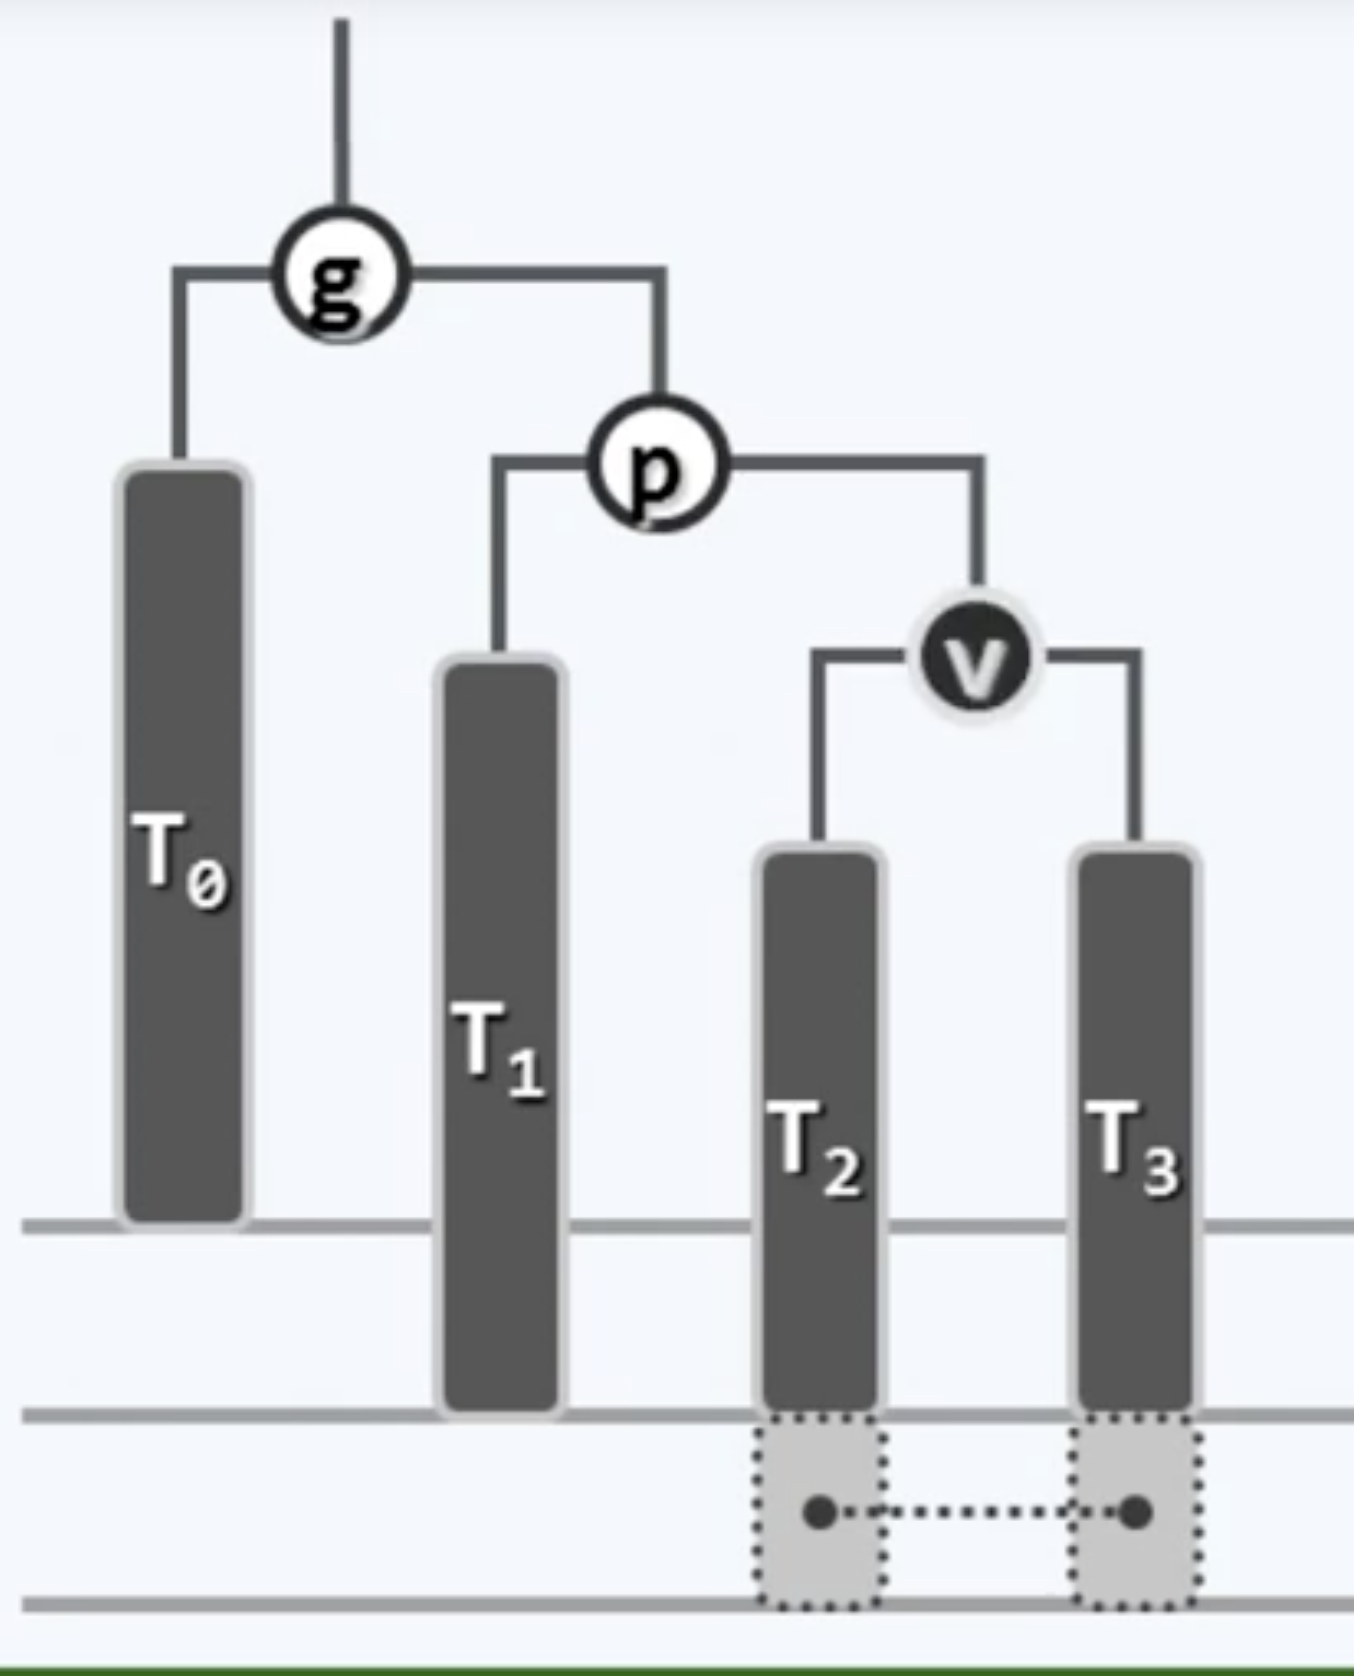
\includegraphics[width=0.4\columnwidth]{insert_rotate_before.png}
    %/caption{before}
  }
  \quad
  \subfigure[rotating]{
    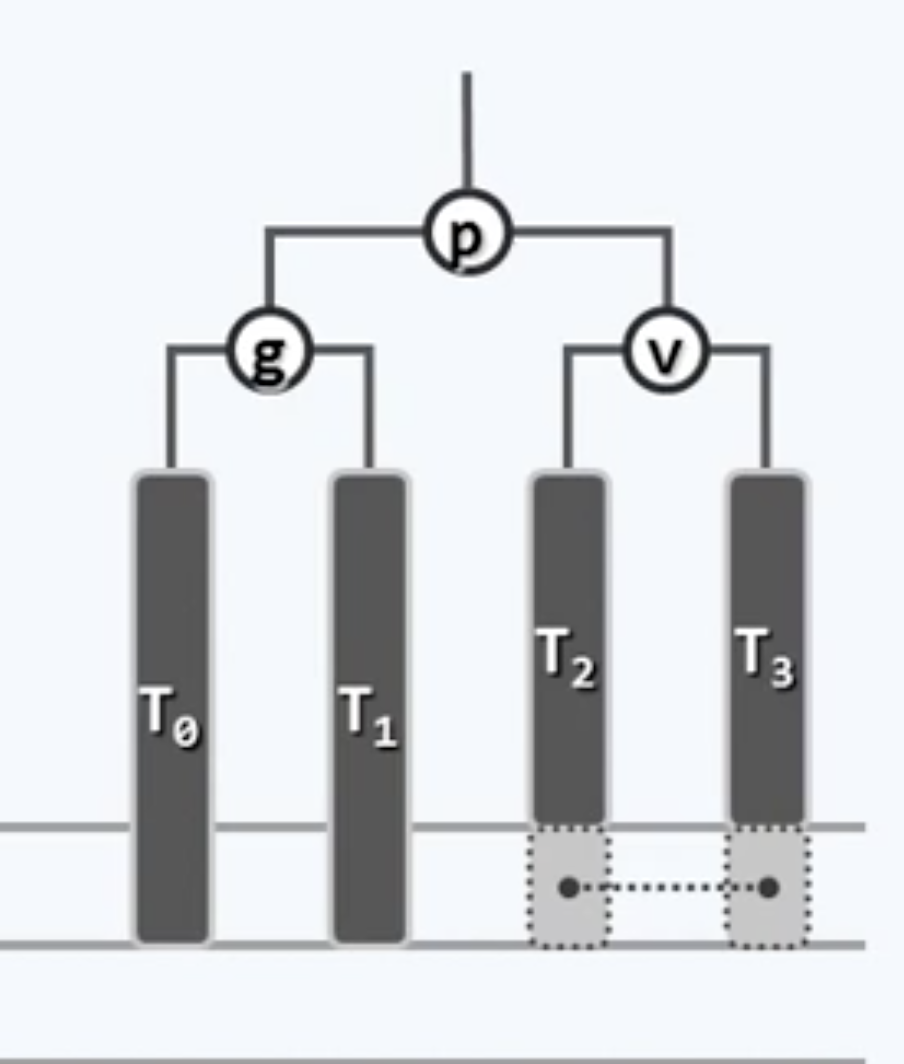
\includegraphics[width=0.4\columnwidth]{insert_rotate_ing.png}
    %/caption{rotating}
  }
  \quad
  \subfigure[after]{
    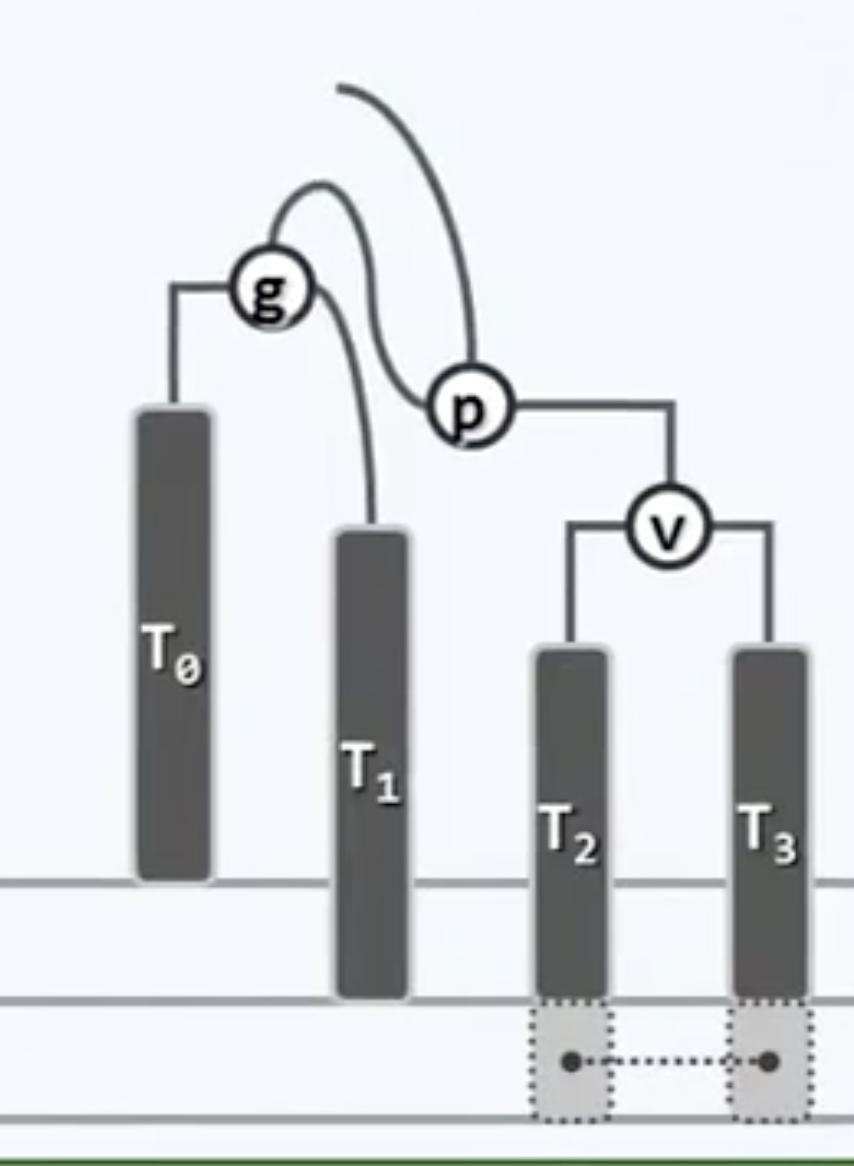
\includegraphics[width=0.4\columnwidth]{insert_rotate_after.png}
    %/caption{after}
  }
  \label{insert_rotate}
\end{figure}

\end{document}
